\documentclass[12pt]{article}

\usepackage[margin=1in]{geometry}
\usepackage{amsmath, amssymb, amsthm}
\usepackage{graphicx}
\usepackage{booktabs}
\usepackage{hyperref}
\usepackage{natbib}
\usepackage{setspace}
\usepackage{caption}
\usepackage{float}

\onehalfspacing

\title{Simulating Homo Moralis:\\
Preference Evolution in the Prisoners' Dilemma}
\author{}
\date{}

\begin{document}

\maketitle

\begin{abstract}
\noindent
This report replicates and extends the key results of \citet{AlgerWeibull2013}
through numerical simulation. We focus on the Prisoners' Dilemma (PD) to
illustrate the paper's central claim: when matching is assortative with index
$\sigma$, the evolutionarily stable preference is \emph{homo moralis} with
Kantian coefficient $\kappa = \sigma$. We verify the closed-form equilibrium
cooperation levels and confirm convergence of replicator dynamics to the
predicted fixed point $\kappa = \sigma$ for four values of assortativity.
\end{abstract}

%-----------------------------------------------------------------------
\section{Introduction}
%-----------------------------------------------------------------------

A central question in economics and evolutionary biology is what preferences
natural selection favors when individuals interact strategically. The canonical
answer---\emph{homo oeconomicus}, pure self-interest---rests on two assumptions:
preferences are observable and matching is uniform random. \citet{AlgerWeibull2013}
relax both. When preferences are \emph{private information} and the matching
process exhibits \emph{assortativity} (similar types are more likely to be
paired), they show that evolution does not favor pure selfishness. Instead, the
evolutionarily stable preference is a one-parameter family they call
\emph{homo moralis}, which blends self-interest with a Kantian moral motive.

The \textbf{Kantian coefficient} $\kappa \in [0,1]$ parameterises this blend.
An individual with coefficient $\kappa$ maximises
\begin{equation}
    u_\kappa(x,y) = (1-\kappa)\,\pi(x,y) + \kappa\,\pi(x,x),
    \label{eq:homo_moralis}
\end{equation}
where $\pi(x,y)$ is the fitness payoff from playing strategy $x$ against an
opponent playing $y$, and $\pi(x,x)$ is the payoff if \emph{everyone} played
$x$---the Kantian ``categorical imperative.'' At $\kappa=0$ the agent is homo
oeconomicus; at $\kappa=1$ the agent is homo kantiensis (pure moralist).

The paper's main theorem states that the unique evolutionarily stable type (under
mild regularity conditions) is \emph{homo hamiltonensis}: homo moralis with
$\kappa = \sigma$, where $\sigma$ is the \textbf{index of assortativity} of the
matching process. This creates a clean, empirically testable mapping: more
assortative environments (family, tight communities) should produce more moral
behavior.

This report replicates the paper's results numerically using two exercises:
(i) the equilibrium cooperation correspondence in the PD as a function of
$\kappa$, and (ii) replicator dynamics over a population of types to confirm
convergence to $\kappa = \sigma$.

%-----------------------------------------------------------------------
\section{Model}
%-----------------------------------------------------------------------

\subsection{Prisoners' Dilemma}

A strategy $x \in [0,1]$ denotes the probability of cooperation. Using the
paper's payoff parameters ($T=7, R=5, P=3, S=2$, satisfying $T>R>P>S$), the
expected payoff function is
\begin{equation}
    \pi(x,y) = xyR + x(1-y)S + (1-x)yT + (1-x)(1-y)P.
\end{equation}
This is bilinear in $x$ and $y$:
\begin{equation}
    \pi(x,y) = Axy + Bx + Cy + D,
    \quad A = R-S-T+P,\; B=S-P,\; C=T-P,\; D=P.
\end{equation}

\subsection{Homo Moralis Equilibrium in the PD}

A homo moralis with coefficient $\kappa$ maximises $u_\kappa(x,y)$ in
\eqref{eq:homo_moralis}. In the symmetric Nash equilibrium both players choose
$x^*(\kappa)$. \citet{AlgerWeibull2013} derive the closed form:
\begin{equation}
    x^*(\kappa) = \begin{cases}
        0            & \kappa \leq \kappa_L, \\
        \hat{x}(\kappa) & \kappa_L < \kappa < \kappa_H, \\
        1            & \kappa \geq \kappa_H,
    \end{cases}
    \label{eq:xstar}
\end{equation}
where the thresholds and interior solution are
\begin{equation}
    \kappa_L = \frac{P-S}{T-P} = 0.25, \qquad
    \kappa_H = \frac{T-R}{R-S} = 0.67,
\end{equation}
\begin{equation}
    \hat{x}(\kappa)
    = \frac{S + \kappa T - (1+\kappa)P}{(1+\kappa)(S+T-R-P)}.
\end{equation}
The equilibrium cooperation level is strictly increasing in $\kappa$ over the
interior region and jumps to corners at the two thresholds.

\subsection{Fitness and Evolutionary Stability}

In a two-type population with resident type $\kappa$ (share $1-\varepsilon$)
and rare mutant $\kappa'$ (share $\varepsilon$), the average fitness functions
in the limit $\varepsilon \to 0$ are
\begin{align}
    \Pi_{\text{res}} &= (1-\sigma)\,\pi(x,x) + \sigma\,\pi(x,x) = \pi(x,x), \\
    \Pi_{\text{mut}} &= (1-\sigma)\,\pi(y,x) + \sigma\,\pi(y,y),
\end{align}
where $x = x^*(\kappa)$ and $y = x^*(\kappa')$. More generally, the average
fitness of type $\kappa_i$ against the current population distribution
$\{s_j\}$ is
\begin{equation}
    \Pi_i = \sigma\,\pi(x_i,x_i)
            + (1-\sigma)\sum_j s_j\,\pi(x_i,x_j).
    \label{eq:fitness}
\end{equation}
The bilinear structure of $\pi$ allows \eqref{eq:fitness} to be written as
\begin{equation}
    \Pi_i = \sigma\,\pi(x_i,x_i)
            + (1-\sigma)\bigl[x_i(A\bar{x}+B) + C\bar{x} + D\bigr],
    \quad \bar{x} = \sum_j s_j x_j,
\end{equation}
which is computable from the single aggregate $\bar{x}$ and requires no loop
over types---the key to an efficient simulation.

\subsection{Replicator Dynamics}

We discretise $\kappa$ into $N=200$ equally spaced types on $[0,1]$ and
initialise shares uniformly: $s_i(0) = 1/N$. The replicator update is
\begin{equation}
    s_i(t+1) = s_i(t)\;\frac{\Pi_i(t)}{\bar{\Pi}(t)},
    \quad \bar{\Pi}(t) = \sum_j s_j(t)\,\Pi_j(t).
\end{equation}
All $\sigma$ values are run simultaneously in one loop via NumPy broadcasting
for computational efficiency.

%-----------------------------------------------------------------------
\section{Results}
%-----------------------------------------------------------------------

\subsection{PD Equilibrium Correspondence}

Figure~\ref{fig:pd} plots $x^*(\kappa)$ against $\kappa$ using the closed form
in \eqref{eq:xstar}. The curve is zero for $\kappa \leq 0.25$ (full defection,
as in standard game theory), rises monotonically through the interior, and
reaches full cooperation for $\kappa \geq 0.67$. The coloured dots mark the
predicted evolutionarily stable cooperation levels for four values of $\sigma$.
Higher assortativity maps directly to higher equilibrium cooperation.

\begin{figure}[H]
    \centering
    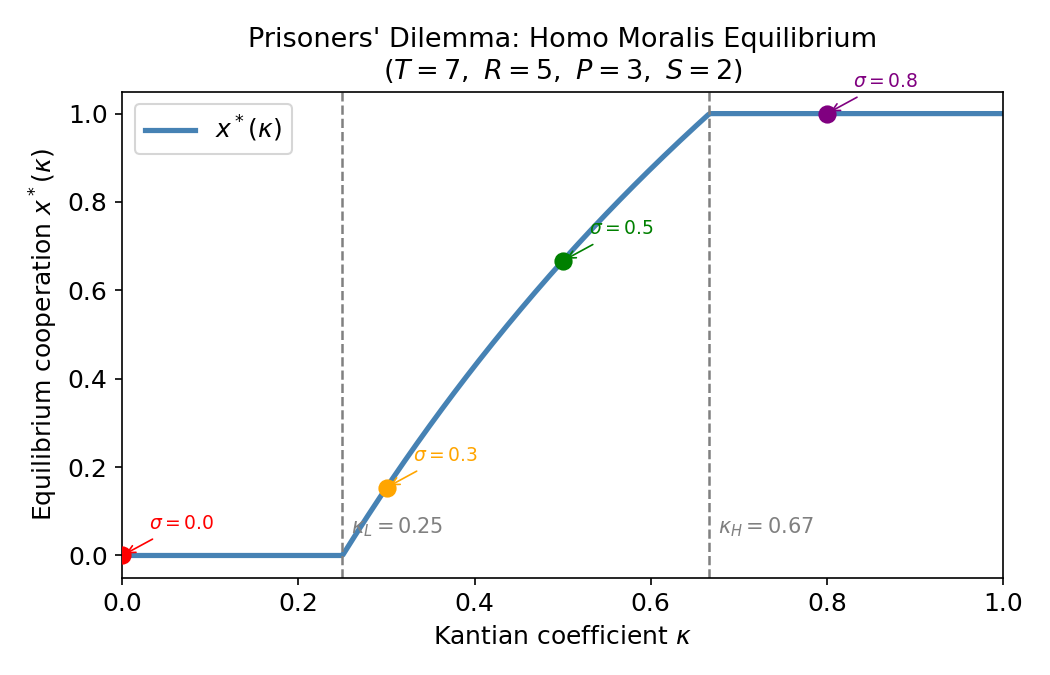
\includegraphics[width=0.75\textwidth]{Code/pd_equilibrium.png}
    \caption{Equilibrium cooperation $x^*(\kappa)$ as a function of the Kantian
    coefficient. Thresholds $\kappa_L = 0.25$ and $\kappa_H = 0.67$ delimit the
    interior region. Coloured dots mark the evolutionarily stable cooperation
    level $x^*(\sigma)$ for each assortativity value $\sigma$.}
    \label{fig:pd}
\end{figure}

\noindent\textbf{Remark on degeneracy.}
The paper's convergence prediction is unambiguous only when $\sigma$ is in the
interior region $(\kappa_L, \kappa_H) = (0.25, 0.67)$. For $\sigma \leq 0.25$
all types $\kappa \in [0, \sigma]$ play $x^* = 0$ and are strategically
identical, so the replicator cannot distinguish among them. The same degeneracy
applies for $\sigma \geq 0.67$. We therefore restrict the evolutionary
simulation to $\sigma \in \{0.3, 0.4, 0.5, 0.6\}$ where the ESS prediction
is non-degenerate.

\subsection{Evolutionary Dynamics}

Figure~\ref{fig:final} shows the population distribution over $\kappa$ after
5,000 generations for each $\sigma$ value. In all four cases, the mass
concentrates in a tight spike whose peak aligns precisely with the predicted
ESS at $\kappa = \sigma$ (dashed line). Table~\ref{tab:results} reports the
mean $\kappa$ of the final distribution.

\begin{figure}[H]
    \centering
    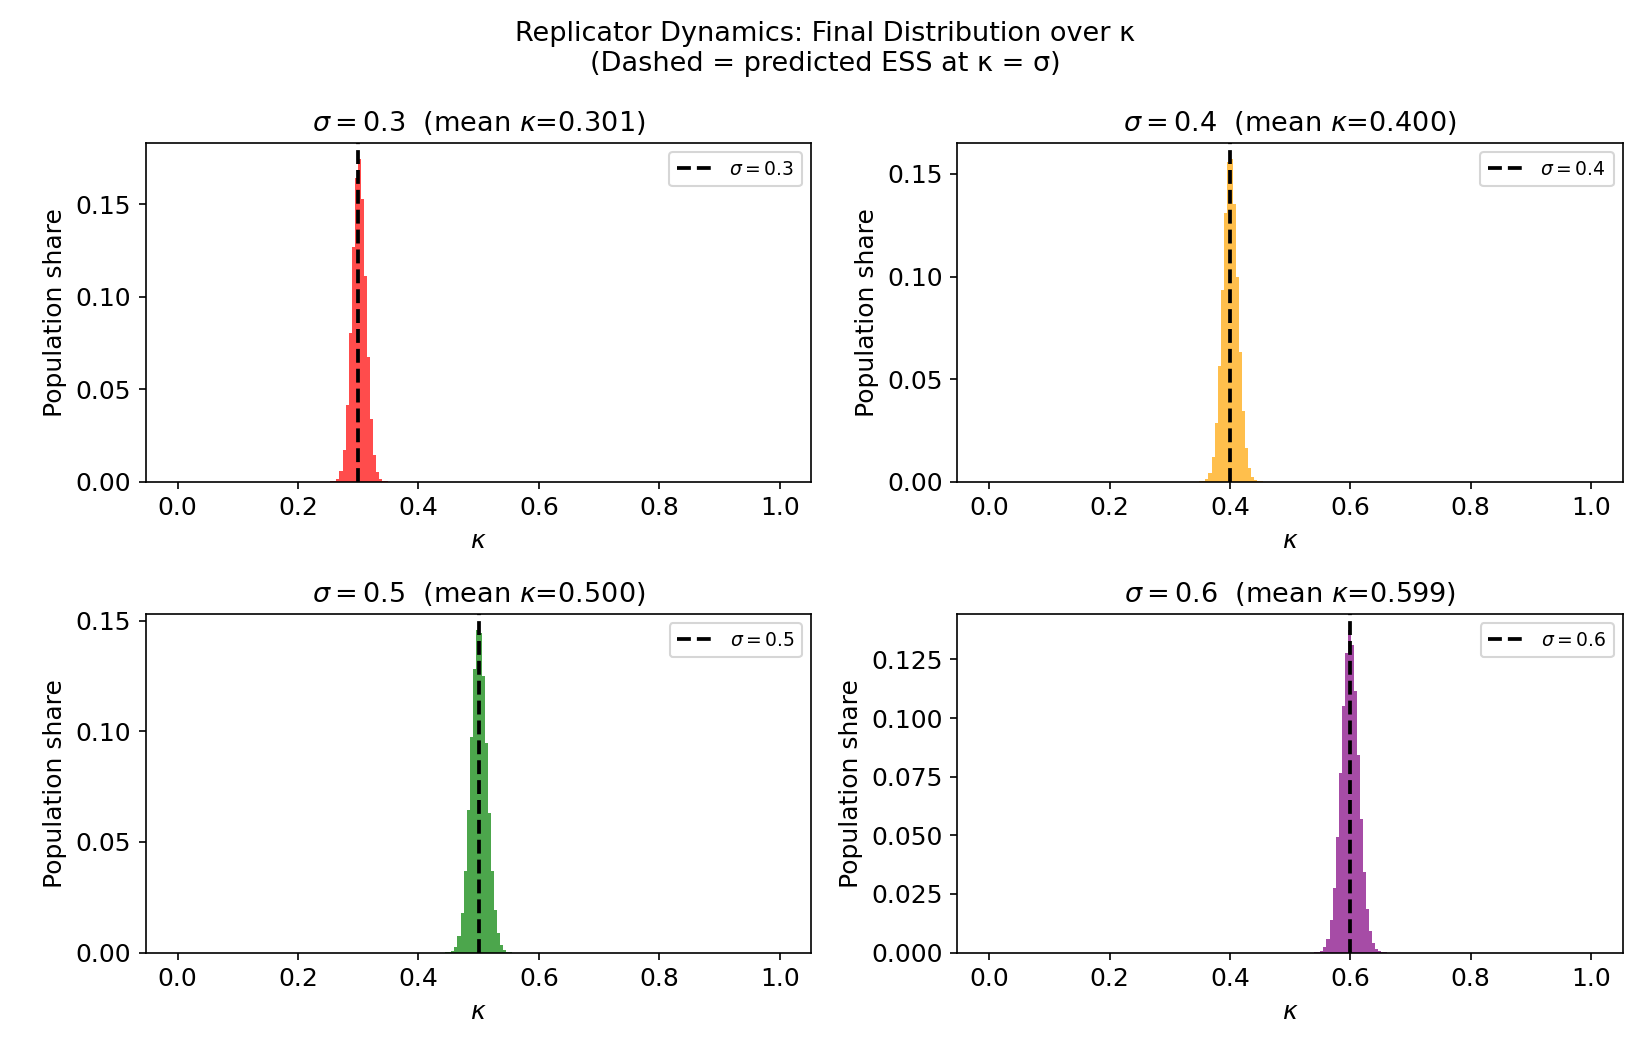
\includegraphics[width=\textwidth]{Code/replicator_final.png}
    \caption{Final population distribution over $\kappa$ after 5,000 generations
    of replicator dynamics, for four values of the assortativity index $\sigma$.
    The dashed line marks the predicted ESS at $\kappa = \sigma$.}
    \label{fig:final}
\end{figure}

\begin{table}[H]
    \centering
    \caption{Predicted ESS vs.\ simulated mean $\kappa$ at generation 5,000.}
    \label{tab:results}
    \begin{tabular}{ccc}
        \toprule
        $\sigma$ & Predicted $\kappa^*$ & Simulated mean $\kappa$ \\
        \midrule
        0.3 & 0.300 & 0.301 \\
        0.4 & 0.400 & 0.400 \\
        0.5 & 0.500 & 0.500 \\
        0.6 & 0.600 & 0.599 \\
        \bottomrule
    \end{tabular}
\end{table}

Figure~\ref{fig:convergence} shows the time path of the mean $\kappa$ for each
$\sigma$. All four trajectories converge to their respective targets, confirming
the paper's ESS result. Convergence is fastest for $\sigma = 0.4$ and
$\sigma = 0.5$, which are furthest from the boundary thresholds and thus face
the strongest fitness gradient. Cases near the boundaries ($\sigma = 0.3$
near $\kappa_L$, $\sigma = 0.6$ near $\kappa_H$) take around 3,000--4,000
generations to settle.

\begin{figure}[H]
    \centering
    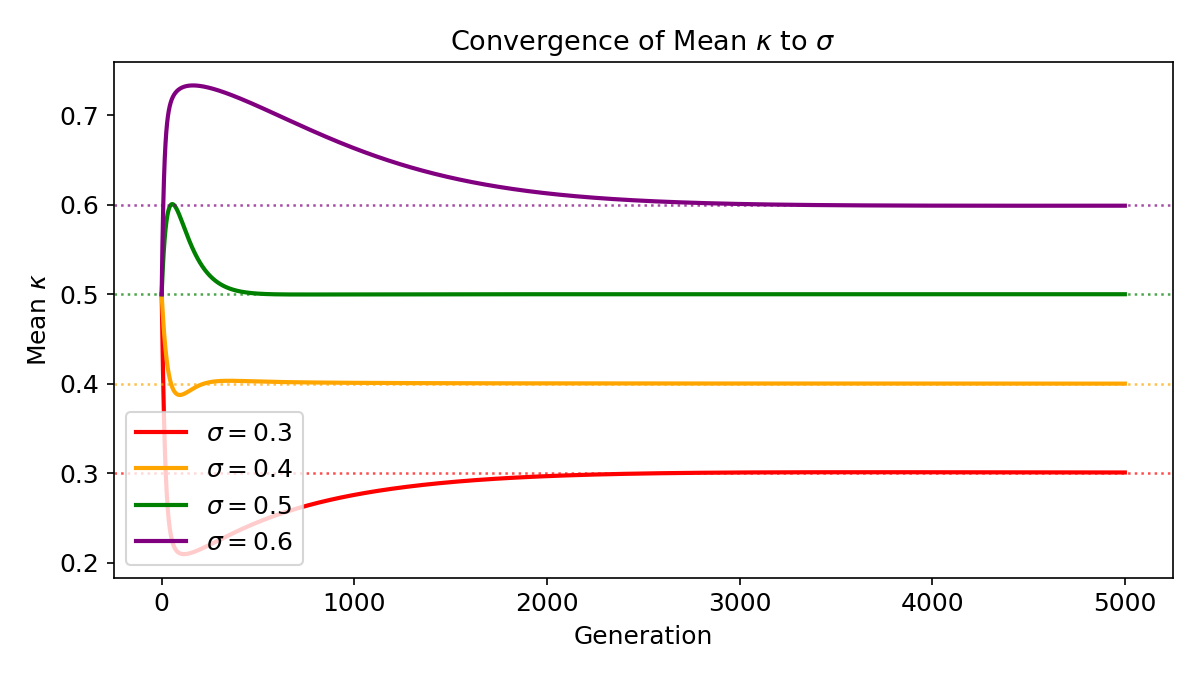
\includegraphics[width=0.85\textwidth]{Code/replicator_convergence.png}
    \caption{Mean $\kappa$ in the population over time. Dotted lines mark the
    predicted limits $\sigma$. All trajectories converge to $\kappa = \sigma$.}
    \label{fig:convergence}
\end{figure}

Figure~\ref{fig:heatmap} provides a detailed view for $\sigma = 0.5$,
plotting the full population density over $\kappa$ and time. Initially the
distribution is uniform. Within roughly 100 generations the mass begins
concentrating around $\kappa = 0.5$; by generation 500 the spike is clearly
formed and tightens thereafter.

\begin{figure}[H]
    \centering
    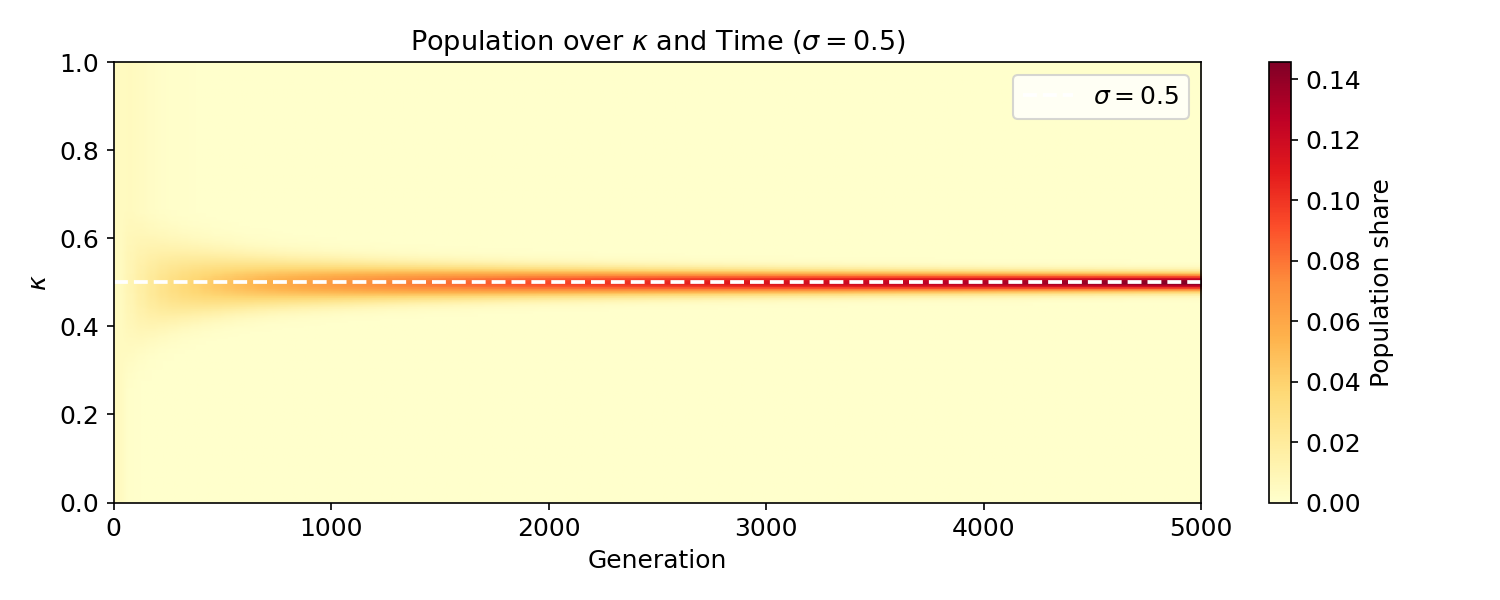
\includegraphics[width=\textwidth]{Code/replicator_heatmap.png}
    \caption{Population density over $\kappa$ and time for $\sigma = 0.5$.
    Colour intensity indicates population share. The white dashed line marks
    the predicted ESS at $\kappa = 0.5$.}
    \label{fig:heatmap}
\end{figure}

%-----------------------------------------------------------------------
\section{Conclusion}
%-----------------------------------------------------------------------

The simulation confirms the central theorem of \citet{AlgerWeibull2013}.
Starting from a uniform distribution of preference types, replicator dynamics
converge to a point mass at $\kappa = \sigma$---the degree of morality equals
the index of assortativity. Three implications stand out:

\begin{enumerate}
    \item \textbf{Morality is endogenous to the matching environment.} The
    degree of Kantian morality that survives evolutionary selection is
    determined entirely by $\sigma$, not by the payoff structure of the
    fitness game.

    \item \textbf{Higher assortativity sustains more cooperation.} In the PD,
    $x^*(\sigma)$ is strictly increasing in $\sigma$ over the interior region.
    Tight communities and kin-based interactions generate higher equilibrium
    cooperation as a direct consequence of evolutionary pressure.

    \item \textbf{Pure selfishness is generically unstable.} Homo oeconomicus
    ($\kappa = 0$) is only evolutionarily stable when $\sigma = 0$ (uniform
    random matching). Any positive assortativity selects for a strictly positive
    Kantian coefficient.
\end{enumerate}

\bibliographystyle{plainnat}
\bibliography{references}

\end{document}
